\documentclass[12pt]{article}

\usepackage{graphicx}
\usepackage{amsmath}
\usepackage{amsfonts}
\usepackage{float}
\usepackage{subcaption}

\usepackage{pseudocode}
\usepackage{listings}
\usepackage{color}

\usepackage{ifthen}
\usepackage{seqsplit}

\usepackage{qcircuit}
\usepackage{braket}

\usepackage{enumerate}
\usepackage{enumitem}
\usepackage{scrextend}
\usepackage{pdfpages}

\usepackage{tikz}
\usetikzlibrary{trees}

\DeclareMathOperator{\Tr}{Tr}
\DeclareMathOperator{\ord}{ord}

\addtolength{\textwidth}{1in}
\addtolength{\textheight}{1in}
\addtolength{\evensidemargin}{0.5in}
\addtolength{\oddsidemargin}{-0.5in}
\addtolength{\topmargin}{-0.5in}

\title{Cooperative Agents in Euchre}
\author{Taras Mychaskiw}
\date{April 16th, 2015}

\begin{document}
\maketitle

    \begin{abstract}
        Typically, agents use a set of rules or follow a specific strategy when given options in order to maximize their expected utility.
        This project explores such a setting in the card game euchre. Euchre gives an interesting setting where two teams of two agents
        compete in an incomplete information game. A suite of euchre playing agents are given which each follow a specific
        and quick strategy in order to maximize not only their personal utility, but their team utility.
    \end{abstract}
    
    \thispagestyle{empty}
    \clearpage
    \thispagestyle{empty}
    \tableofcontents
    \clearpage
    \setcounter{page}{1}
    
    
\section{Introduction}
% talk about related work here

A good heuristic or static evaluation function in games helps an agent make decisions which maximize their utility. This idea
works well, however in team settings, maximizing a personal score may not be a good team strategy. In this project, we
investigate this setting in the card game euchre, where two teams of two complete to maximize their team score. Some agents
show, among those studied, that cooperation is a much more powerful strategy. This idea was defined in the prisoner's dilemma, where
two rational agents that maximize their personal score end up both losing. If these agents cooperated instead, their personal scores
and ``team'' scores would be optimal.

Card games remain popular to study, as their offer interesting settings which lead to good understandings and findings. For example,
a common thread in many card games is that they are incomplete information games -- other players' hands or the deck is not known to
the agent. Perhaps the most interesting about card games is that humans are (generally) much better than the best known artificial agent.
Famously, poker was solved in \cite{poker}, however they study a very small version of poker compared to what is normal in tournament play.
Not to discredit their results, but just to say that much work needs still be done in order for artificial agents to consistently beat the
best human players in many card game settings. Euchre, compared to other card games, is less conventional in that it is also a cooperative game.
This project details various artificial agents for euchre in order to discover a strategy that is superior.

\subsection{Euchre}

Simply put, euchre is a trick taking card game. It plays very similarly to other trick taking games, such as hearts or bridge.
The euchre deck only consists of 24 cards, 9 through ace of each suit. Each of the four players is dealt five cards which makes up
their hand. Each players' hand is only known to them. The 21st card of the deck is turned face up to be offered as trump. The remaining
three cards remain hidden and are not used in the hand (known as the ``kitty'').

Players then take turns deciding on if they wish to ``order up'' the offered trump card. If so, the dealer must pick up the offered card,
place it in his hand and secretly discard a card into the kitty. If the card is not ordered up, players take turns having the option to
call a trump suit or pass -- but players cannot call the same trump suit as what was offered prior. Players can also choose to ``go alone''
when they call a trump suit, which forbids their partner from playing the hand in the hopes of scoring more points.

Once trump is called, the main portion of the game takes place. The player left of the dealer leads the first trick. Each player adds a card
to the trick in turn. The winner of the trick leads the next trick. This play continues for five rounds, until all players are out of cards.
Afterwards, teams count how many trick their won and the team that took at least three of the tricks scores points as:
\begin{itemize}[noitemsep, label={}]
    \item 1 point : if called trump and took 3-4 tricks
    \item 2 points: if called trump and took all 5 tricks
    \item 2 points: if didn't call trump and took 3-5 tricks
    \item 4 points: if went alone and took all 5 tricks
\end{itemize}

This play continues, shifting who deals every hand, until a team scores 10 points. That is euchre in a nutshell -- though trump hasn't been explained.
The general play follows the above guidelines. There are additional rules with trump and which cards you can play into a trick, which are detailed below.

When a player leads a trick, the card they play determines the lead suit of the trick. Other players must play a card of the same suit
if possible, otherwise they can play any card from their hand. The player with the highest ranked card in the trick wins it, however those cards
which are not the lead suit or trump cannot ever win the trick. For example, if I lead the $9\heartsuit$ and you followed with A$\diamondsuit$, my
lowly 9 is still winning the trick because you did not follow suit (assuming $\diamondsuit$ is not trump).

Trump in euchre is peculiar, and leads to much confusion for beginners. For non-trump suits, the rankings of cards is as you would expect, ace $>$
king $>$ queen \ldots. The lowest trump cards beat the highest non-trump cards (easy enough), however the rankings in among trump is not the same as
non-trump. Let $\spadesuit$ be trump for a concrete example. The ordering of trump then goes
J$\spadesuit$ $>$ J$\clubsuit$ $>$ A$\spadesuit$ $>$ K$\spadesuit$ $>$ Q$\spadesuit$ $>$ $10\spadesuit$ $>$ $9\spadesuit$.
The jack is the highest card in the game, followed by the other jack of the same colour -- in our example J$\spadesuit$ is the best and J$\clubsuit$
is the second best (called the ``right'' and ``left'' bowers respectfully). The left bower is the confusing part. Though it is printed J$\clubsuit$, it
becomes a $\spadesuit$ as long as $\spadesuit$ is trump. So when $\clubsuit$ is led and your only $\clubsuit$ is J$\clubsuit$, you are not forced
to play it as it is not a $\clubsuit$, but a $\spadesuit$. Likewise, when $\spadesuit$ is led, you must play J$\clubsuit$ since it is a $\spadesuit$.
This means there are 7 $\spadesuit$ in the game, 6 of each $\diamondsuit$ and $\heartsuit$ and only 5 $\clubsuit$.
Similarly when a red suit is called trump, the other red jack becomes the left bower and it becomes on the trump suit rather than it's printed suit.


\subsection{Agent Considerations}

With the rules of euchre in mind, we can consider what information is known and important to an artificial agent. When it comes times to play a card
into a trick, the following information is known:
\begin{itemize}[noitemsep, label={}]
    \item the rules of euchre
    \item their own hand
    \item the card offered as trump
    \item all of the cards played so far, and by whom
    \item the trump suit
    \item the lead suit of the trick, is any
    \item the overall rankings of each card
\end{itemize}

This is all the information an agent has access to. Additional information can be inferred, such as when a player doesn't follow the lead suit,
it is known that the player cannot possibly have any cards of that suit in their hand (assuming they are not cheating). Making the best use of
all the information available will lead to a powerful euchre agent. In the next section, we introduce several euchre agents which make
different uses of all this available information. Afterwards, we compare these strategies to each other to determine which is best among them.
Lastly, we will discuss the strengths and weaknesses of particular strategies and conclude with ideas for future work.

    
    
\section{Euchre Agents}

The overall objective in euchre is to take as many tricks as possible. This ensures the other team does not benefit from them.
Generally, this strategy works well, but it ignores the team aspect of the game. In this section, we give several euchre strategies
making various use of the information available in the game. All agents know the basic rules of the game, as a useful agent could
not be constructed without this knowledge. Additionally, no agent can cheat. When we say an agent chooses to play a card with some
property, it is assumed that the card is chosen from the set of legally playable cards. These strategies range from simple to selfish to
complex. These strategies aimed to produce a very quick (near instant in most cases) but good decision when playing a card from
their hand into a trick.


\subsection{Simple Strategies}

The first strategies discussed will be very simple, but serve as a very good base for more complex strategies. These agents only make use
of the information given directly to them, their hand. The first agent plays a random card from their hand. This agent exists to serve
as a basis for comparison. The next two agents are opposites of each other, one always plays the lowest card in their hand while
the other always plays the highest card. Since these agents do not use any additional information, they all play selfishly.

The agents High and Low serve as an excellent foundation for more complex agents. In euchre, the overall goal is to maximize the number
of tricks your team earns. Playing High will give you the best possible chance of winning a trick, while Low allows you to throw away
your worst card if you resign a trick. Playing a ``Middle'' strategy would not help compared to High and Low as it seems to give you
the worst traits of both the other strategies. With Middle, you could have an increased chance of taking a trick, but if you lost the trick,
you've lost a decent card which could have been used later to win a different trick. Due to this, no Middle agent was explored.


\subsection{More Complex Strategies}

The next agents become slightly more complex. These agents make use of the information given to them in the trick. The first one,
called HighLow, behaves as follows:
\begin{itemize}[noitemsep, label={}]
    \item if I have a card that can win the trick, play High
    \item otherwise, there's no hope, play Low
\end{itemize}
This HighLow strategy proves to perform quite well, and makes a lot of sense. If it is possible to take a trick, playing the best card
gives the highest chance of actually winning the trick. If there's no hope of winning a trick, playing your worst card
saves your better cards in the hopes that they can win later tricks.

A cooperative version of HighLow was created as well, called CoopHighLow. The logic of this agent is as follows:
\begin{itemize}[noitemsep, label={}]
    \item if partner has played in the trick and is winning, play Low
    \item otherwise, play HighLow
\end{itemize}
This strategy aims to not take tricks from your partner if it can be avoided. If your partner is winning the trick, saving your good cards for
later and allowing them to win will generally be a very powerful strategy. However, if your partner is losing the trick, or hasn't played,
the semi-aggressive HighLow strategy makes sense to play to try to win tricks or avoid losing better cards.


\subsection{Markov Decision Strategy}

The next agent uses a simplified Markov decision process to determine it's hand strength compared to the strength of remaining cards.
The agent uses the ratio of these values to guess at whether a card in his hand is strong and has a good chance of winning the trick.
At a high level, the Markov agent keeps track of all cards that have been seen and it knows what cards have not been seen. A value is
assigned to each card in the deck which represents the strength of that card. When it comes time to make a decision, the Markov agent
performs:
\begin{equation}
    \text{action}(H, D, \tau) = \left\{ \begin{array}{lr}
            \text{play High} & : \frac{Value(H)}{Value(U \setminus D)} \geq \tau \\
            \text{play Low}  & : \frac{Value(H)}{Value(U \setminus D)} < \tau 
        \end{array} \right. \nonumber
\end{equation}
where $H$ is the set of cards in the agent's hand, $D$ is the set of cards that have been seen and $U$ is the set of all cards. The function
$Value(\cdot)$ gives the sum of the values of all the cards in the given set. The threshold parameter $\tau$ determines the operating point
of the agent. As $\tau$ grows, the Markov agent becomes more aggressive. Essentially, when the Markov agent sees a high ratio value,
it deems it's hand as good and a High card is played. Otherwise, a lwo values is viewed as weak and a Low card is played.

The specific values for $\tau$ and the cards used in our experiments are discussed in the next section.


\subsection{Card Counting Strategy}

The CardCounting agent tries to use all available information to it's advantage. This agent keeps track of whether or not each player can
possibly have a card or not. When a card is seen, it is known that no player can possibly hold that card in their hand, so this information
is tracked. For additional information, whenever a player does not follow the lead suit, it is known that the player cannot have any of the
lead suit in their hand. This information is also recorded.

In addition to using all available information, this agent employs a different strategy depending on how many cards are in the trick.
It tries to use players being out of a suit or strong in a suit to the team advantage. At a high level, the CardCounting agent performs
the following thought process before making a decision:

\begin{itemize}[label={}]
    \item \textbf{Leading the trick}
        \begin{itemize}[noitemsep]
            \item if partner is out of a suit and has trump, play Low in that suit hoping the partner can play trump
            \item if partner is ``strong'' in a suit compared to both other players, play Low in that suit
            \item otherwise, play High
        \end{itemize}
    \item \textbf{Second to play}
        \begin{itemize}[noitemsep]
            \item if partner can possibly win and is ``stronger'' than the other remaining player, play Low
            \item if partner doesn't have the lead suit:
                \begin{itemize}[noitemsep, label={}]
                    \item if trump was led, play HighLow
                    \item otherwise, if partner has trump, play Low
                \end{itemize}
            \item otherwise, play HighLow
        \end{itemize}
    \item \textbf{Third to play}
        \begin{itemize}[noitemsep]
            \item if partner is winning so far but the last player can win the trick, play HighLow
            \item otherwise, play CoopHighLow
        \end{itemize}
    \item \textbf{Last to play}
        \begin{itemize}[noitemsep]
            \item play CoopHighLow
        \end{itemize}
\end{itemize}

This method introduces complexity in the hopes of intelligent performance. This agent aims to maximize the number of tricks the team wins
through trying to let the partner take as many tricks as possible; except when the partner cannot help, where this agent tries to play selfishly
for the benefit of the team.

The word ``strong'' comes up in the above explanation. The strength of a player in a suit is defined as the sum of the ranks of
each card that player can possible have of that suit, where a high ranking means a stronger card. Then, $S_a > S_b$ implies that player $a$
has a stronger hand than player $b$ in that suit.

\subsection{Hybrid Strategy}

The Hybrid strategy combines the logics of the CoopHighLow, Markov and CardCounting agents. Essentially, this agent using the same Markov decision
process as the Markov agent, except when the agent's hand is good, the CoopHighLow strategy is played. Other times, the CardCounting strategy is played.
This strategy was created to hopefully compensate for the passive play of the CardCounting agent with the aggressive behaviour of the CoopHighLow agent.

\subsection{Monte Carlo Agent}

An overly simple strategy in euchre (or any card game) would be to simulate all possible games which follow from the current game state. In incomplete
information settings such as euchre, this is simply not computationally feasible. Instead of traversing the entire game tree, the MonteCarlo agent
randomly traverses the game tree for a set amount of time, keeping track of how many tricks were won in each path. This is similar to the strategy
laid out in \cite{skat}.

To help reduce the search space further, the MonteCarlo agent retains the idea from the CardCounting agent to keep track of which cards every
other player can possibly have. When it comes time to make a decision, a random possible hand is assigned to each other player and games are
simulated until finished. This process is repeated until some amount of time has passed, then the card that led to the most number of trick
wins is played. At the start of a game, this agent will likely perform poorly as the game tree is still enormous, while nearing the end of the
game, the game tree shrinks to a point where it is possible to simulate all possible games which will greatly strengthen play.


    
    
\section{Agent Comparisons}

For each table in this section, we compare two of the strategies discussed in the previous section. At first, we look at
teams where the two agents follow the same strategy, followed later by teams consisting of two different types of agents.
Unless otherwise noted, all the statistics were taken from a simulation of 10,001 games. In these games, it was forced
that the dealer call trump to be $\spadesuit$ for simplicity, as the agents do not have a strategy for calling trump.
This setup might be considered unfair to the dealing team, but all players share the disadvantage and aim to make the best
out of the situation they find themselves in. Given enough games, the disadvantages will even out.
Each game was played until a team had 10 points (teams can get 11 points if they score 2 points when they are at 9 points).

Each agent was also timed when making it's decisions. However, each of these made over 500,000 decisions and the slowest
agent took about 3 seconds to make all these decisions. Due to this, the timings won't be included as they are indistinguishable
during play against a human. With exception of course to the MonteCarlo agent, where each decision is given a set amount of time.


\subsection{Simple Strategies}

The simple strategies were compared to each other. Figures \ref{fig:results_low} and \ref{fig:results_random} show the results of their competition.
As to be expected, Low did poorly overall. Low managed to still win some games however, since Low essentially keeps it's highest cards for the
end of the game. When they get a lucky deal, they can manage to scrape together enough tricks to win a hand. Generally though, playing Low is
worse than playing Random. On the other hand, playing High proved to be slightly better than playing Random, though not by very much.
Also not surprising is that High beats Low, likely due to winning early tricks. Each of the simple agents perform very quickly, each performing
their decisions in very little time.

\begin{figure}[h]
    \centering
    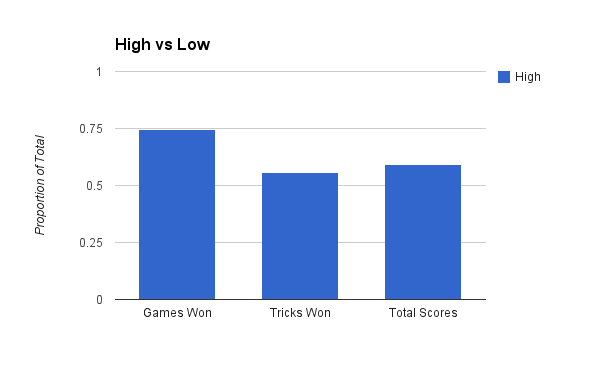
\includegraphics[scale=0.5]{data/low.png}
    \caption{Results of the Low agent against the High agent.}
    \label{fig:results_low}
\end{figure}

\begin{figure}[h]
    \centering
    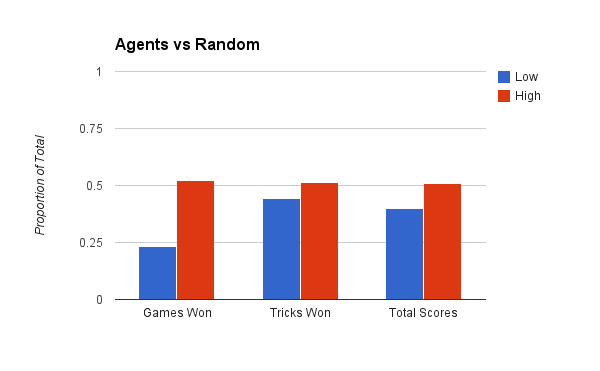
\includegraphics[scale=0.5]{data/random.png}
    \caption{Results of the Random agent against other agents.}
    \label{fig:results_random}
\end{figure}

\subsection{More Complex Strategies}

Figure \ref{fig:results_highlow} show the results for the HighLow agent against the simple strategies. The results show a staggering
favour for the HighLow agent, able to win handily against any of the simple strategies.

Figure \ref{fig:results_coophighlow} show the results for the CoopHighLow agent against the other strategies. Following the trend of 
the HighLow agent, the CoopHighLow proves to be very powerful compared to the simple strategies. This also shows the results of an
important competition. The CoopHighLow and HighLow agents both prove strong agents, but only one of the tries to cooperate with
their team mate. The results favour the CoopHighLow agent, who took on average about a point more per game.

\begin{figure}[h]
    \centering
    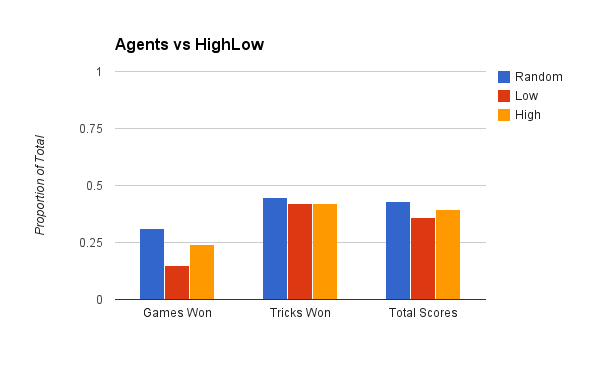
\includegraphics[scale=0.5]{data/highlow.png}
    \caption{Results of the HighLow agent against other agents.}
    \label{fig:results_highlow}
\end{figure}

\begin{figure}[h]
    \centering
    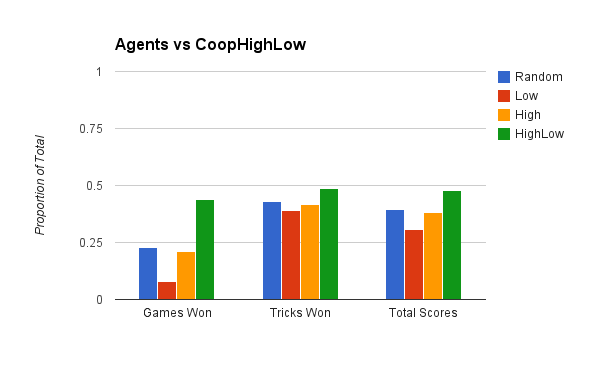
\includegraphics[scale=0.5]{data/coophighlow.png}
    \caption{Results of the CoopHighLow agent against other agents.}
    \label{fig:results_coophighlow}
\end{figure}


\subsection{Markov Decision Strategy}

Here, we show the results of two different Markov agents. They follow the same strategy, however the values they assign to each card
is different. The first agent uses the number of tricks a card wins out of all possible tricks given the current trump suit as the value for
each card. This proved to perform strangely, so an additional value base was formed. Markov2 uses a very similar value base; the value of
a card is the number of tricks the card can win which derive from the current trick and given the trump suit. This different value
base lends itself more closely to the actual values of the cards. For example, an ace that isn't the lead suit or trump cannot win any tricks,
so it should be considered a powerful card. When leading a trick, Markov2 behaves identically to Markov. Both Markov agents used a threshold $\tau$
of 0.25 due to there being 4 players in the game.

Something worth mentioning, these Markov strategies precomputed all the values of the cards and stored them for quick lookup when needed during
the games. They perform much faster this way, but used quite a bit of memory (around 1GB). However, the time taken to precompute the values
was only on the order of a second or two, so in real games they can be calculated on the fly quickly enough.

As mentioned, Markov performs strangely. Markov proves worse than Random, but slightly better than both Low and High. This is strange due to
the results shown in Figure \ref{fig:results_random}, showing that High is better than Random. When played against HighLow and CoopHighLow, Markov
did not do well at all, losing most of the games and averaging relatively low scores.

\begin{figure}[h]
    \centering
    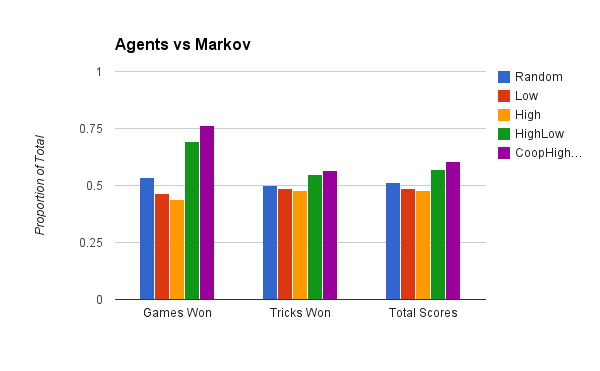
\includegraphics[scale=0.5]{data/markov.png}
    \caption{Results of the Markov agent against other agents.}
    \label{fig:results_markov}
\end{figure}

The Markov2 agent shows more promise than the Markov agent, showing it is actually slightly better than Random and still better
than both High and Low. Markov2 also is quite a bit better than the Markov agent.

This high that Markov2 experienced is quickly brought down by the soul crushing HighLow and CoopHighLow agents. Although Markov2
performed much better than Markov against these two agents, Markov2 was still trounced. Rather unfortunate.

\begin{figure}[h]
    \centering
    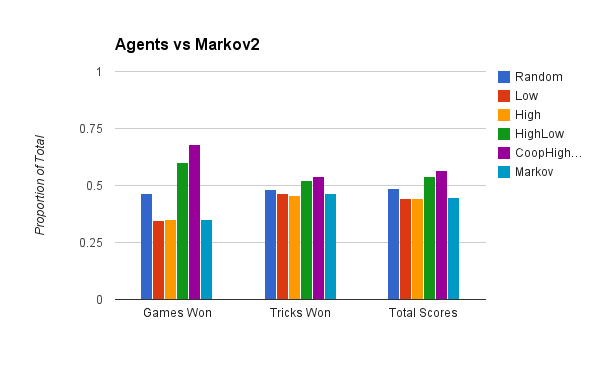
\includegraphics[scale=0.5]{data/markov2.png}
    \caption{Results of the Markov2 agent against other agents.}
    \label{fig:results_markov2}
\end{figure}


\subsection{Card Counting Strategy}

The CardCounting was modelling off of how I personally play euchre, for the most part. Human players tend to keep track of what suit
players hold and play accordingly. The CardCounting, similar to the HighLow agent, performs very well against the simple strategies.
The results are promising, as the agent achieves very high average scores in each game.


Surprisingly, the more complex strategy modelled after more human play performs not as well as expected against the relatively simple
CoopHighLow agent. CardCounting was able to beat the HighLow agent. However, against the CoopHighLow agent, the CardCounting
essentially tied, performing slightly worse but taking more tricks. It is due to this disappointing result that the Hybrid strategy
was created, in hopes to beat the CoopHighLow agent.

As shown in the previous subsection, the Markov agents are not very powerful. They are swept aside by the CardCounting agent.

\begin{figure}[h]
    \centering
    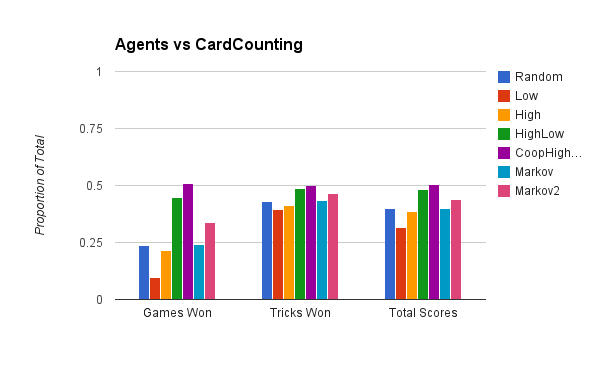
\includegraphics[scale=0.5]{data/cardcounting.png}
    \caption{Results of the CardCounting agent against other agents.}
    \label{fig:results_cardcounting}
\end{figure}


\subsection{Hybrid Strategy}

how the hybrid works


again, how disappointing


although the hybridization worked much better than cardcounting

\begin{figure}[h]
    \centering
    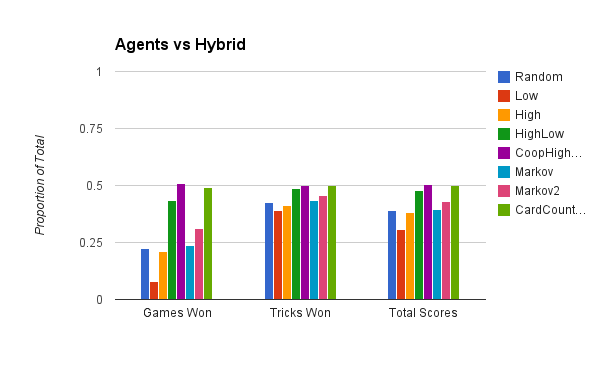
\includegraphics[scale=0.5]{data/hybrid.png}
    \caption{Results of the Hybrid agent against other agents.}
    \label{fig:results_hybrid}
\end{figure}

since markov2 worked so well, hybrid2


what is this nonsense


better than cardcounting again, worse than hybrid

\begin{figure}[h]
    \centering
    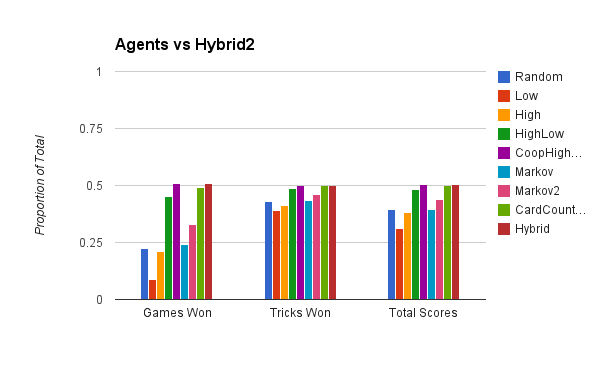
\includegraphics[scale=0.5]{data/hybrid2.png}
    \caption{Results of the Hybrid2 agent against other agents.}
    \label{fig:results_hybrid2}
\end{figure}



\subsection{Monte Carlo Agent}



\subsection{Mixed Agent Teams}


    
    
\section{Discussion}


\subsection{Strengths of Particular Agents}


\subsection{Weaknesses of Particular Agents}

cardcounting fails to check for enemies missing suits

montecarlo sucks at beginning which leads to a bad ending


    
    
\section{Conclusions and Future Work}

This project aimed to create an intelligent euchre playing agent, but found that relatively simple strategies performed
just as well if not better than more complex ones. This leads to the conclusion that euchre is mostly not about trick taking,
but about trump calling. Unfortunately, none of the strategies given are able to call a meaningful trump suit. This is not to say
that CoopHighLow, the best performing agent overall, is an optimal trick taking euchre strategy. On the contrary, we have given some
weaknesses that the CoopHighLow strategy has and ways to improve upon them.

Some future work would be to create a more complete rule set for the CardCoutning agent to improve it. This would in turn improve
the Hybrid agent. Further improvements can be made to Hybrid, the parameters can be learned instead of arbitrarily assigned, perhaps
leading to a much better agent overall. Perhaps the learned values can be used to make an intelligent decision when calling trump.
Additionally, a more complex Markov decision process can be used instead of a simple threshold.

In this project, several trick taking euchre strategies are given. A simple rule base consisting of Random, High and Low build
up into more complex and more powerful agents. Counter intuitively, a relatively simple strategy proves to be the best trick taker
out of those studied. Though it is not a perfect strategy, it can serve as an excellent foundation for future trick taking strategies.
This result leads to the conclusion that trick taking is euchre is not as difficult as the decision to call trump, when very little
about the state of the game is known.

All of the source code for this project is freely available at\\https://github.com/twentylemon/euchre

    
    \bibliographystyle{plain}
    \bibliography{euchre}

\end{document}
